%%%%%%%%%%%%%%%%%%%%%%%%%%%%%%%%%%%%%%%%%
% Beamer Presentation
% LaTeX Template
% Version 1.0 (10/11/12)
%
% This template has been downloaded from:
% http://www.LaTeXTemplates.com
%
% License:
% CC BY-NC-SA 3.0 (http://creativecommons.org/licenses/by-nc-sa/3.0/)
%
%%%%%%%%%%%%%%%%%%%%%%%%%%%%%%%%%%%%%%%%%

%----------------------------------------------------------------------------------------
% PACKAGES AND THEMES
%----------------------------------------------------------------------------------------

\documentclass[12pt,xcolor={dvipsnames}]{beamer}
%\setbeamersize{text margin left=1em,text margin right=1em}
\usepackage{mathtools}
\usepackage{amsmath}
\usepackage{bm}
\usepackage{hyperref}

\usepackage{graphicx} % Allows including images
\graphicspath{{/Users/rebecca/Documents/JER/MinimiseMatrixJER/MCvsData_PowhegPythia/}{/Users/rebecca/Documents/JER/MinimiseMatrixJER/}{/Users/rebecca/Documents/JER/MinimiseMatrixJER/PowhegPythiavsSherpa/}{/Users/rebecca/Documents/Presentations/Talks/}}
\usepackage{booktabs} % Allows the use of \toprule, \midrule and \bottomrule in tables

\usepackage{etoolbox}

\usepackage{subcaption}
\captionsetup{compatibility=false}

\usepackage{multirow}

\usepackage{appendixnumberbeamer}

%\newlength\origleftmargini
%\setlength\origleftmargini\leftmargini
%\setbeamertemplate{itemize/enumerate body begin}{\setlength{\leftmargini}{2pt}}%

%\let\oldexampleblock\exampleblock
%\let\oldendexampleblock\endexampleblock
%\def\exampleblock{\begingroup \setbeamertemplate{itemize/enumerate body begin}{\setlength{\leftmargini}{\origleftmargini}} \oldexampleblock}
%\def\endexampleblock{\oldendexampleblock \endgroup}%

%\let\oldalertblock\alertblock
%\let\oldendalertblock\endalertblock
%\def\alertblock{\begingroup \setbeamertemplate{itemize/enumerate body begin}{\setlength{\leftmargini}{\origleftmargini}} \oldalertblock}
%\def\endalertblock{\oldendalertblock \endgroup}

\mode<presentation> {

% The Beamer class comes with a number of default slide themes
% which change the colors and layouts of slides. Below this is a list
% of all the themes, uncomment each in turn to see what they look like.

%\usetheme{default}
%\usetheme{AnnArbor}
%\usetheme{Antibes}
%\usetheme{Bergen}
%\usetheme{Berkeley}
%\usetheme{Berlin}
\usetheme{Boadilla}
%\usetheme{CambridgeUS}
%\usetheme{Copenhagen}
%\usetheme{Darmstadt}
%\usetheme{Dresden}
%\usetheme{Frankfurt}
%\usetheme{Goettingen}
%\usetheme{Hannover}
%\usetheme{Ilmenau}
%\usetheme{JuanLesPins}
%\usetheme{Luebeck}
%\usetheme{Madrid}
%\usetheme{Malmoe}
%\usetheme{Marburg}
%\usetheme{Montpellier}
%\usetheme{PaloAlto}
%\usetheme{Pittsburgh}
%\usetheme{Rochester}
%\usetheme{Seahorse}
%\usetheme{Singapore}
%\usetheme{Szeged}
%\usetheme{Warsaw}

% As well as themes, the Beamer class has a number of color themes
% for any slide theme. Uncomment each of these in turn to see how it
% changes the colors of your current slide theme.

%\usecolortheme{albatross}
%\usecolortheme{beaver}
%\usecolortheme{beetle}
%\usecolortheme{crane}
%\usecolortheme{dolphin}
%\usecolortheme{dove}
%\usecolortheme{fly}
%\usecolortheme{lily}
%\usecolortheme{RoyalBlue}
%\usecolortheme{rose}
%\usecolortheme{seagull}
%\usecolortheme{seahorse}
%\usecolortheme{whale}
%\usecolortheme{wolverine}

%%Changing the theme colours
%\setbeamercolor*{structure}{bg=Plum!20,fg=Plum}
%\setbeamercolor*{palette primary}{use=structure,fg=white,bg=structure.fg}
%\setbeamercolor*{palette secondary}{use=structure,fg=white,bg=structure.fg!75}
%\setbeamercolor*{palette tertiary}{use=structure,fg=white,bg=structure.fg!50!black}
%\setbeamercolor*{palette quaternary}{fg=white,bg=black}
%\setbeamercolor{section in toc}{fg=black,bg=white}
%%\setbeamercolor{alerted text}{use=structure,fg=structure.fg!50!black!80!black}
%\setbeamercolor{titlelike}{parent=palette primary,fg=structure.fg!50!black}
%\setbeamercolor{frametitle}{bg=gray!30!white,fg=Plum}
%\setbeamercolor*{titlelike}{parent=palette primary}

%Changing the theme colours
\setbeamercolor*{structure}{bg=RoyalPurple,fg=RoyalPurple}
\setbeamercolor*{palette primary}{use=structure,fg=white,bg=structure.fg}
\setbeamercolor*{palette secondary}{use=structure,fg=white,bg=structure.fg}
\setbeamercolor*{palette tertiary}{use=structure,fg=white,bg=structure.fg}
\setbeamercolor*{palette quaternary}{fg=white,bg=black}
\setbeamercolor{section in toc}{fg=black,bg=white}
%\setbeamercolor{alerted text}{use=structure,fg=structure.fg!50!black!80!black}
\setbeamercolor{titlelike}{parent=palette primary,fg=structure.fg!50!black}
%\setbeamercolor{frametitle}{use=structure,fg=white,bg=structure.fg}
\setbeamercolor*{titlelike}{parent=palette primary}

%\setbeamercolor{block}{bg=yellow!10,fg=black}
%\setbeamercolor{block title}{bg=yellow!50,fg=black}
%\AtBeginEnvironment{block}{\setbeamercolor{itemize item}{fg=yellow}}

\newenvironment<>{examplefirst}[1]{%
  \setbeamercolor{block title}{bg=yellow!50,fg=black}%
  \begin{block}#2{#1}}{\end{block}}
\AtBeginEnvironment{examplefirst}{\setbeamercolor{itemize item}{fg=yellow}}

%\setbeamertemplate{footline} % To remove the footer line in all slides uncomment this line
%\setbeamertemplate{footline}[page number] % To replace the footer line in all slides with a simple slide count uncomment this line

%\setbeamertemplate{navigation symbols}{} % To remove the navigation symbols from the bottom of all slides uncomment this line


\setbeamertemplate{blocks}[rounded][shadow=false]
\setbeamertemplate{itemize items}[circle]
\setbeamertemplate{itemize subitems}[circle]

\renewcommand{\thefootnote}{\alph{footnote}}

}

%----------------------------------------------------------------------------------------
% TITLE PAGE
%----------------------------------------------------------------------------------------



\title[Jet Energy Resolution Plots]{Jet Energy Resolution for the Dijet Balance Method} % The short title appears at the bottom of every slide, the full title is only on the title page

\author{\underline{Rebecca Pickles}, Darren Price} % Your name
%\institute[UoM] % Your institution as it will appear on the bottom of every slide, may be shorthand to save space
%{
%University of Manchester\\ % Your institution for the title page
%\medskip
%\textit{julia.iturbe@cern.ch} % Your email address
%}
% logo of my university
\titlegraphic{
\includegraphics[width=3cm]{UniOfManchesterLogo}}
\date{\today} % Date, can be changed to a custom date

\begin{document}


\begin{frame}
\titlepage % Print the title page as the first slide
\end{frame}

\iffalse
\begin{frame}
\frametitle{Overview} % Table of contents slide, comment this block out to remove it
\tableofcontents % Throughout your presentation, if you choose to use \section{} and \subsection{} commands, these will automatically be printed on this slide as an overview of your presentation
\end{frame}
\fi
%----------------------------------------------------------------------------------------
% PRESENTATION SLIDES
%----------------------------------------------------------------------------------------

%------------------------------------------------
\section{Introduction} % Sections can be created in order to organize your presentation into discrete blocks, all sections and subsections are automatically printed in the table of contents as an overview of the talk

%------------------------------------------------
\iffalse

\fi

\begin{frame}
\frametitle{Status}
\begin{itemize}
\item Changed the resolution definition to take into account the difference in asymmetry for the probe and reference rapidity regions:
\newline \newline  $\sigma$(A) = $\sqrt{2}$$\frac{\sigma(p_{T})}{p_{T}}$  \newline \newline $\frac{\sigma(p_{T})}{p_{T}}$ = $\sqrt{4\sigma^{2}(A_{(i,j)})-2\sigma^{2}(A_{(i,i)})}$ \newline
\item Restricted fits for the asymmetry to $\pm$ 0.4 and Nsig = 1.5.
\item Re-ran the subtractions for Powheg+Pythia8, Sherpa, pure Pythia and data
\end{itemize}
\end{frame}

%----------------------------Powheg+Pythia8-----------------------------------

\begin{frame}
\frametitle{Powheg+Pythia8 Truth: Before extra restrictions}
\center
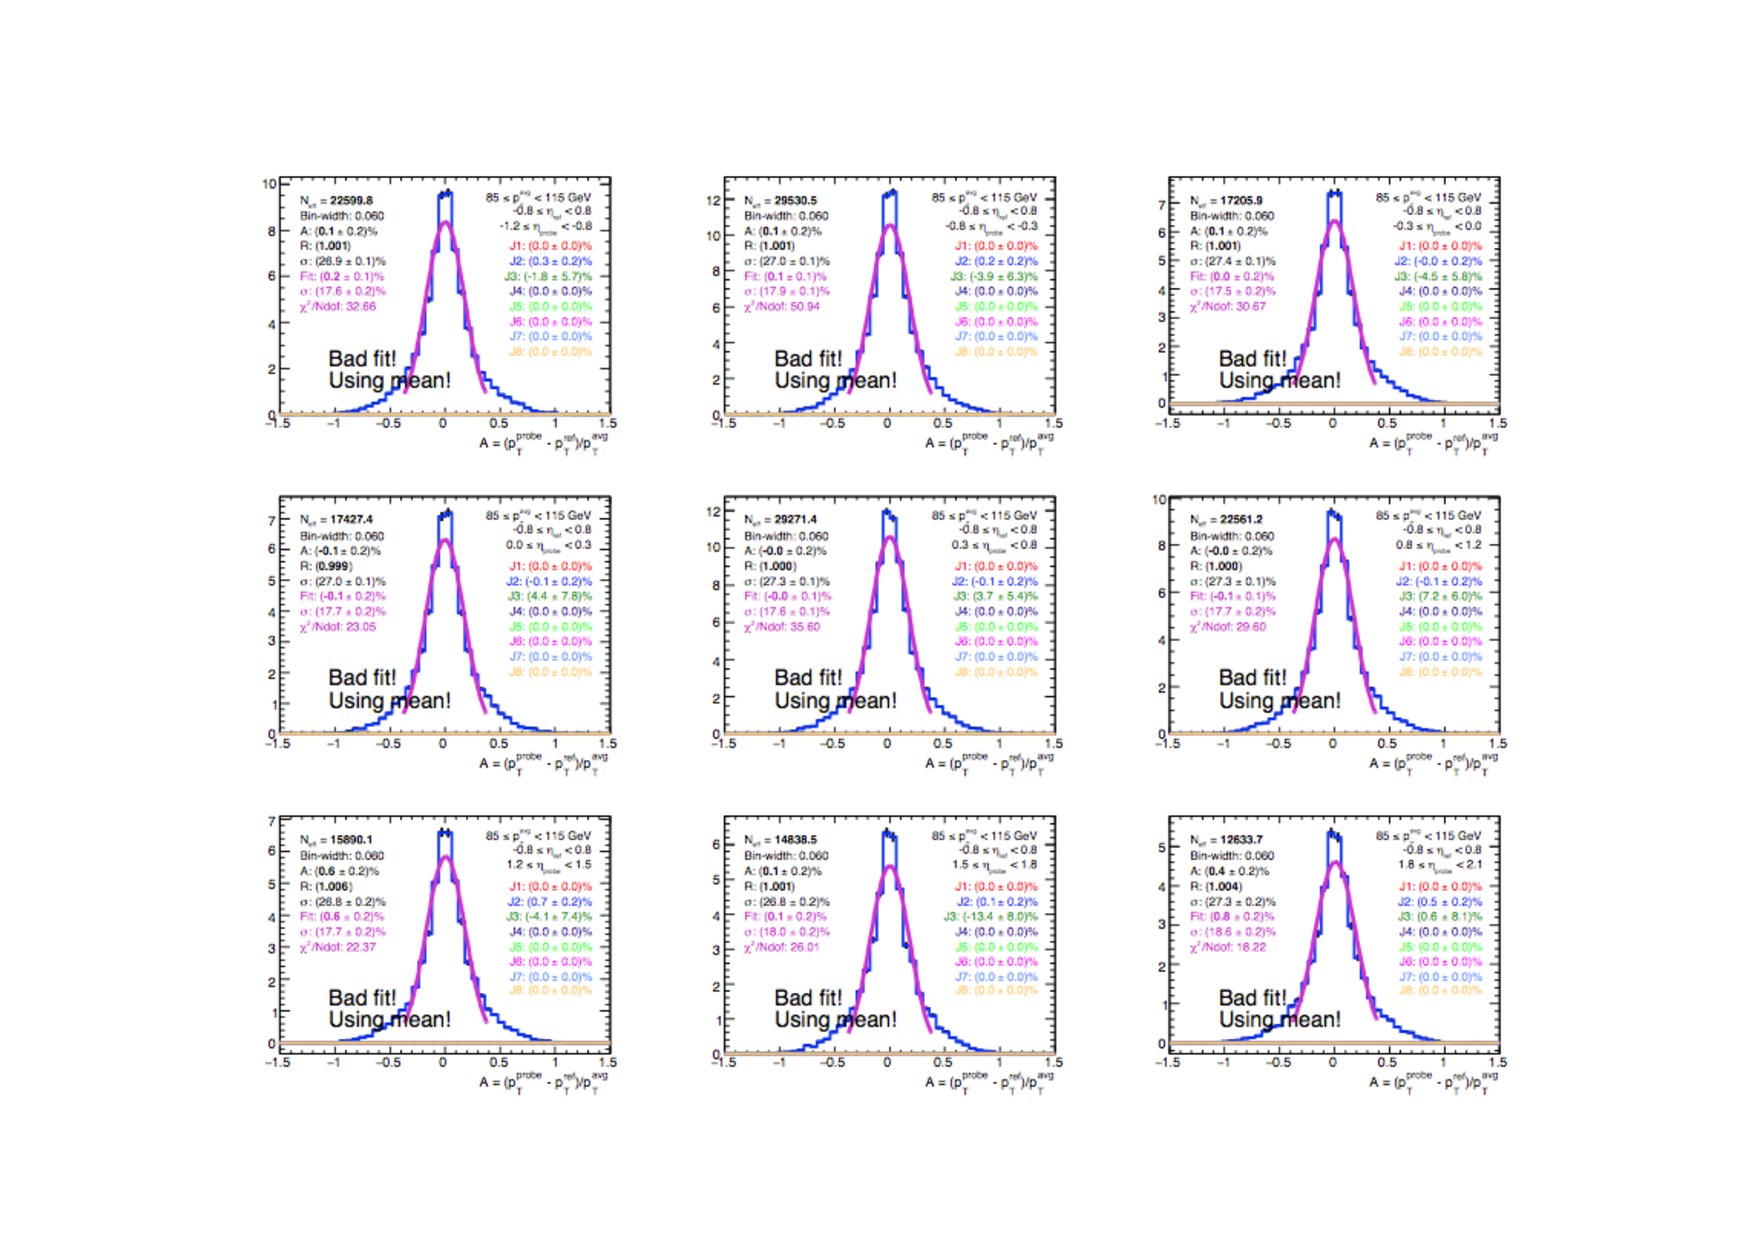
\includegraphics[width=10cm, height=7.5cm]{85to115PPTruthFitsNoRestrict1.pdf}
\end{frame}

\begin{frame}
\frametitle{Powheg+Pythia8 Truth: After restrictions}
\center
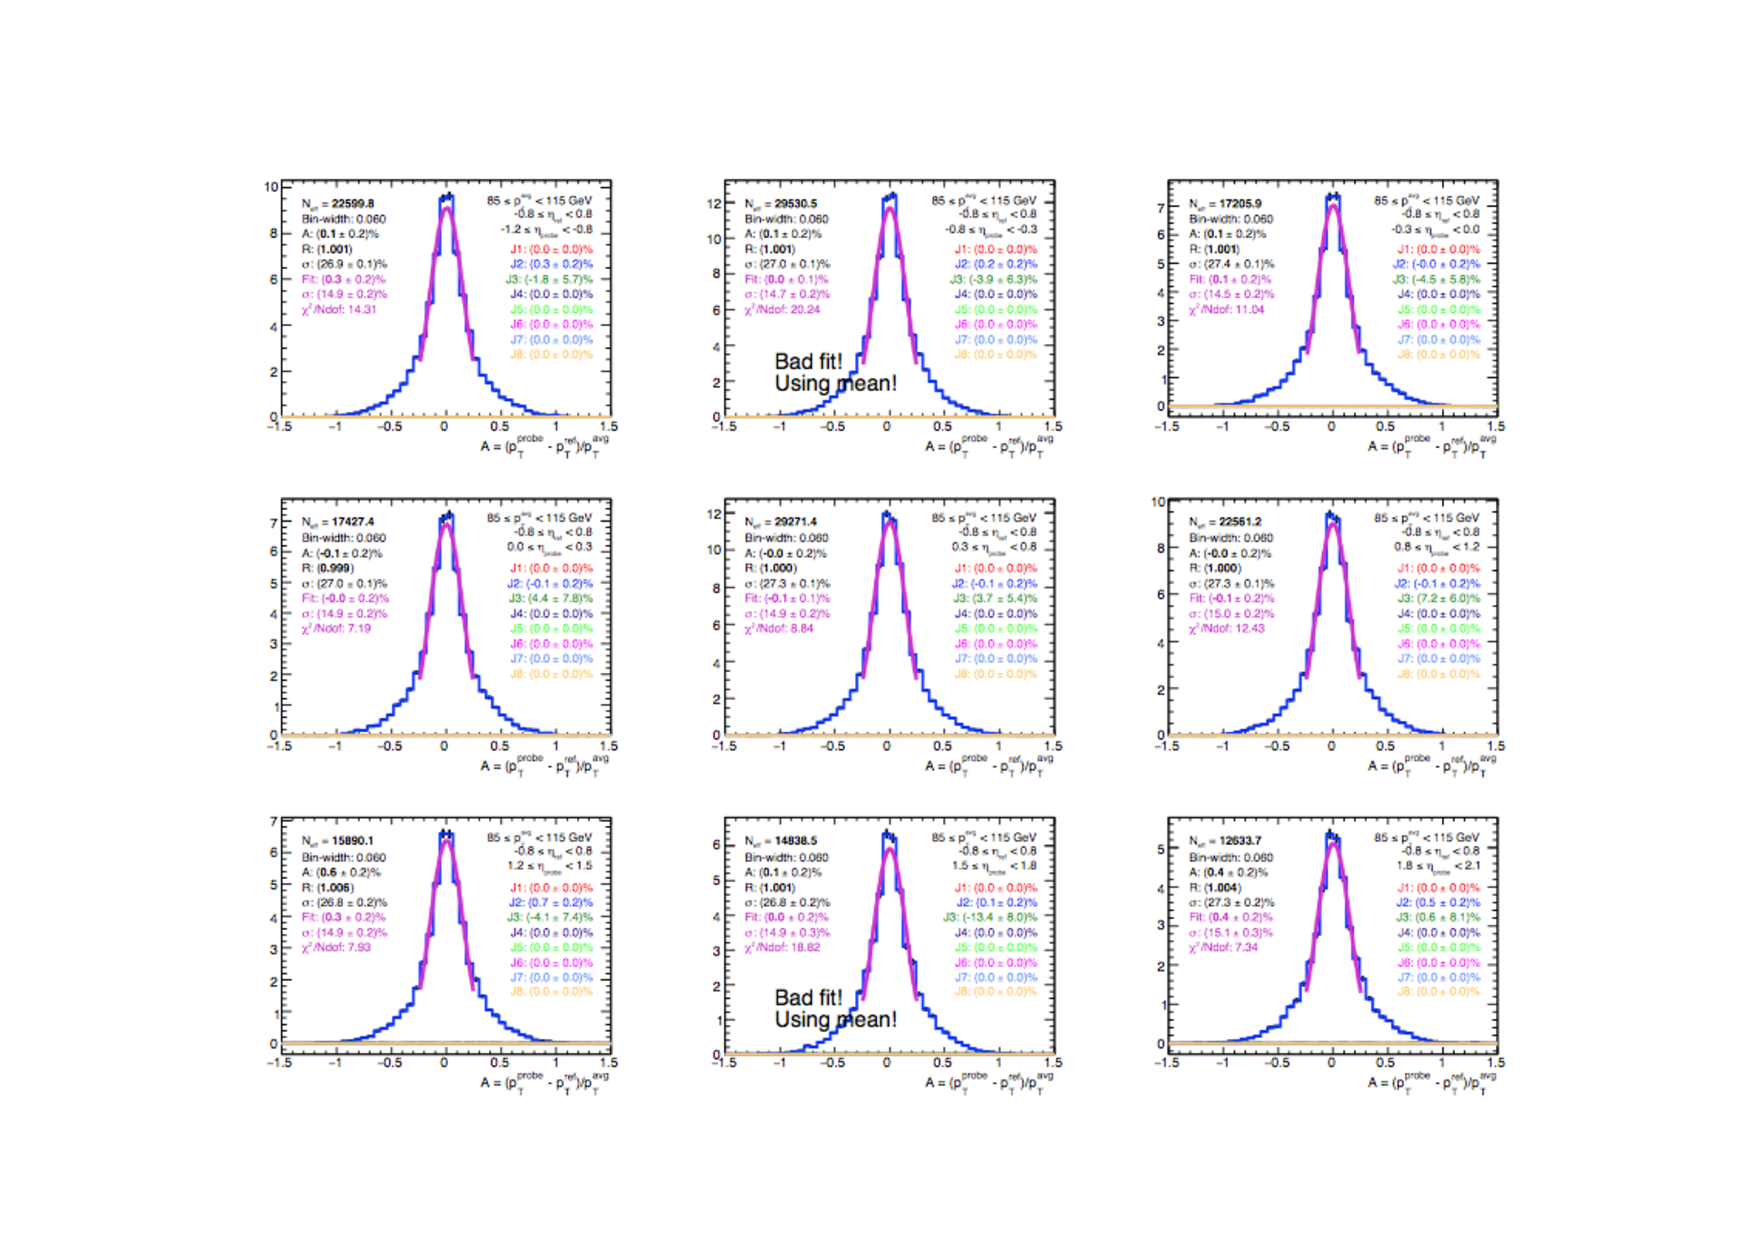
\includegraphics[width=10cm, height=7.5cm]{85to115PPTruthFits0415_1.pdf}
\end{frame}


\begin{frame}
\frametitle{Powheg+Pythia8 unsubtracted $\sigma$($P_{T}$)/$P_{T}$}
\begin{columns}
\begin{column}{.4\textwidth}
\includegraphics[width=4.5cm, height=3cm]{MCvsData_PowhegPythia/25pTavg40_MCvsData.pdf}
\newline
\includegraphics[width=4.5cm, height=3cm]{MCvsData_PowhegPythia/145pTavg175_MCvsData.pdf}
\end{column}
\begin{column}{.4\textwidth}
\includegraphics[width=4.5cm, height=3cm]{MCvsData_PowhegPythia/220pTavg270_MCvsData.pdf}
\newline
\includegraphics[width=4.5cm, height=3cm]{MCvsData_PowhegPythia/270pTavg330_MCvsData.pdf}
\end{column}
\end{columns}
Reference region value is higher: Makes sense with subtraction needed for the probe region, but seems physically counter-intuitive?
\end{frame}

\begin{frame}
\frametitle{Powheg+Pythia8 subtracted $\sigma$($P_{T}$)/$P_{T}$}
\begin{columns}
\begin{column}{.4\textwidth}
\includegraphics[width=4.5cm, height=3cm]{Difference_PowhegPythia/25pTavg40_Difference.pdf}
\newline
\includegraphics[width=4.5cm, height=3cm]{Difference_PowhegPythia/145pTavg175_Difference.pdf}
\end{column}
\begin{column}{.4\textwidth}
\includegraphics[width=4.5cm, height=3cm]{Difference_PowhegPythia/220pTavg270_Difference.pdf}
\newline
\includegraphics[width=4.5cm, height=3cm]{Difference_PowhegPythia/270pTavg330_Difference.pdf}
\end{column}
\end{columns}
\begin{itemize}
\item Bump in reference region doesn't quite cancel out - but smaller.
\item Bug in code: some points don't join up - for no apparent reason (Looking in to it)
\end{itemize}
\end{frame}

%--------------------------------Sherpa-------------------------------------------

\begin{frame}
\frametitle{Sherpa unsubtracted $\sigma$($P_{T}$)/$P_{T}$}
\begin{columns}
\begin{column}{.4\textwidth}
\includegraphics[width=4.5cm, height=3cm]{MCvsData_Sherpa/25pTavg40_MCvsData.pdf}
\newline
\includegraphics[width=4.5cm, height=3cm]{MCvsData_Sherpa/145pTavg175_MCvsData.pdf}
\end{column}
\begin{column}{.4\textwidth}
\includegraphics[width=4.5cm, height=3cm]{MCvsData_Sherpa/220pTavg270_MCvsData.pdf}
\newline
\includegraphics[width=4.5cm, height=3cm]{MCvsData_Sherpa/270pTavg330_MCvsData.pdf}
\end{column}
\end{columns}
There are still a number of eta bins of truth higher than Reco after fit restriction 
\end{frame}

\begin{frame}
\frametitle{Sherpa subtracted $\sigma$($P_{T}$)/$P_{T}$}
\begin{columns}
\begin{column}{.4\textwidth}
\includegraphics[width=4.5cm, height=3cm]{Difference_Sherpa/25pTavg40_Difference.pdf}
\newline
\includegraphics[width=4.5cm, height=3cm]{Difference_Sherpa/145pTavg175_Difference.pdf}
\end{column}
\begin{column}{.4\textwidth}
\includegraphics[width=4.5cm, height=3cm]{Difference_Sherpa/220pTavg270_Difference.pdf}
\newline
\includegraphics[width=4.5cm, height=3cm]{Difference_Sherpa/270pTavg330_Difference.pdf}
\end{column}
\end{columns}
\begin{itemize}
\item The truth being larger than the reco means a lack of points on the subtraction plots. (But this is better than before the fit had been restricted)
\item Also, same issue with lack of line connecting points
\end{itemize}
\end{frame}

%-------------------------PurePythia8--------------------------------------

\begin{frame}
\frametitle{Pure Pythia8 unsubtracted $\sigma$($P_{T}$)/$P_{T}$}
\begin{columns}
\begin{column}{.4\textwidth}
\includegraphics[width=4.5cm, height=3cm]{MCvsData_Pythia/25pTavg40_MCvsData.pdf}
\newline
\includegraphics[width=4.5cm, height=3cm]{MCvsData_Pythia/145pTavg175_MCvsData.pdf}
\end{column}
\begin{column}{.4\textwidth}
\includegraphics[width=4.5cm, height=3cm]{MCvsData_Pythia/220pTavg270_MCvsData.pdf}
\newline
\includegraphics[width=4.5cm, height=3cm]{MCvsData_Pythia/270pTavg330_MCvsData.pdf}
\end{column}
\end{columns}
\begin{itemize}
\item Also has a number of eta bins with truth higher than Reco even with restricted fits
\item Bug in code: Causing strange behaviour of reco at central eta region (What could this be due to?)
\end{itemize}
\end{frame}

\begin{frame}
\frametitle{Pure Pythia8 subtracted $\sigma$($P_{T}$)/$P_{T}$}
\begin{columns}
\begin{column}{.4\textwidth}
\includegraphics[width=4.5cm, height=3cm]{Difference_Pythia/25pTavg40_Difference.pdf}
\newline
\includegraphics[width=4.5cm, height=3cm]{Difference_Pythia/145pTavg175_Difference.pdf}
\end{column}
\begin{column}{.4\textwidth}
\includegraphics[width=4.5cm, height=3cm]{Difference_Pythia/220pTavg270_Difference.pdf}
\newline
\includegraphics[width=4.5cm, height=3cm]{Difference_Pythia/270pTavg330_Difference.pdf}
\end{column}
\end{columns}
\begin{itemize}
\item Same Issue as with Sherpa: The truth being larger than the reco means a lack of points on the subtraction plots.
\end{itemize}
\end{frame}



\begin{frame}
\frametitle{To-Do:}
\begin{itemize}
\item How to fix subtraction problem without restricting fits further? (Restricting further causes problems with both truth and reco.)
\item Fix bugs in code causing lack of connecting points and sudden negative values at central eta for Pythia8.
\item Calculate MC detector resolution from:
\newline \newline $\frac{P_{T}^{reco} - P_{T}^{truth}}{P_{T}^{reco}}$
\newline \newline in bins of ($P_{T}^{reco}$, $\eta$) for $\Delta$R matched jets for each MC.
\end{itemize}
\end{frame}




\end{document} 